\chapter{Control Groups}

Cgroup servono a limitare le risorse come ad esempio memoria, cpu, ecc. che sono
a disposizione di un gruppo di processi. Se impostato correttamente, cgroups
evita che un processo tenga tutte le risorse per se anche se sarebbero necessarie
ad altri processi e permette anche di prevenire attacchi come le fork bomb
(creazione di troppi processi).

\section{Gerarchia}

C'è una gerarchia di control group per ogni tipo di risorsa che viene gestita.
Ognuna di queste viene gestita da un \textit{cgroup controller}.
Un qualsiasi processo linux fa parte di un cgroup di ogni tipo e quando un
processo figlio viene creato eredita i cgroup del padre.\\

Il kernel linux comunica le informazioni riguardanti cgroups attraverso un insieme
di più pseudo-filesystem che solitamente risiedono in \verb|/sys/fs/cgroup|.
Effettuando \verb|ls| di quella directory sarà possibile vedere i differenti
tipi di cgroup nel sistema.

\begin{figure}[H]
    \centering
    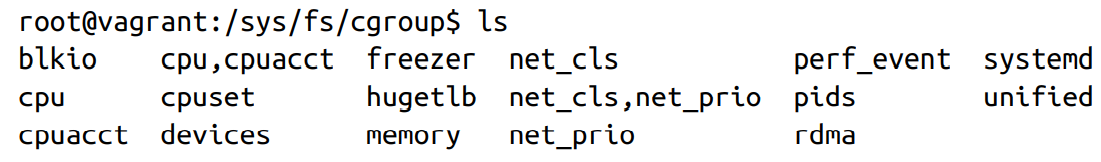
\includegraphics[width=\textwidth, keepaspectratio]{capitoli/os_security/imgs/cgroup1.png}
\end{figure}

La gestione di questi cgroup avviene modificando i file e le directory all'interno
di questa gerarchia. Qui di seguito possiamo vedere un esempio
del cgroup \verb|memory|.

\begin{figure}[H]
    \centering
    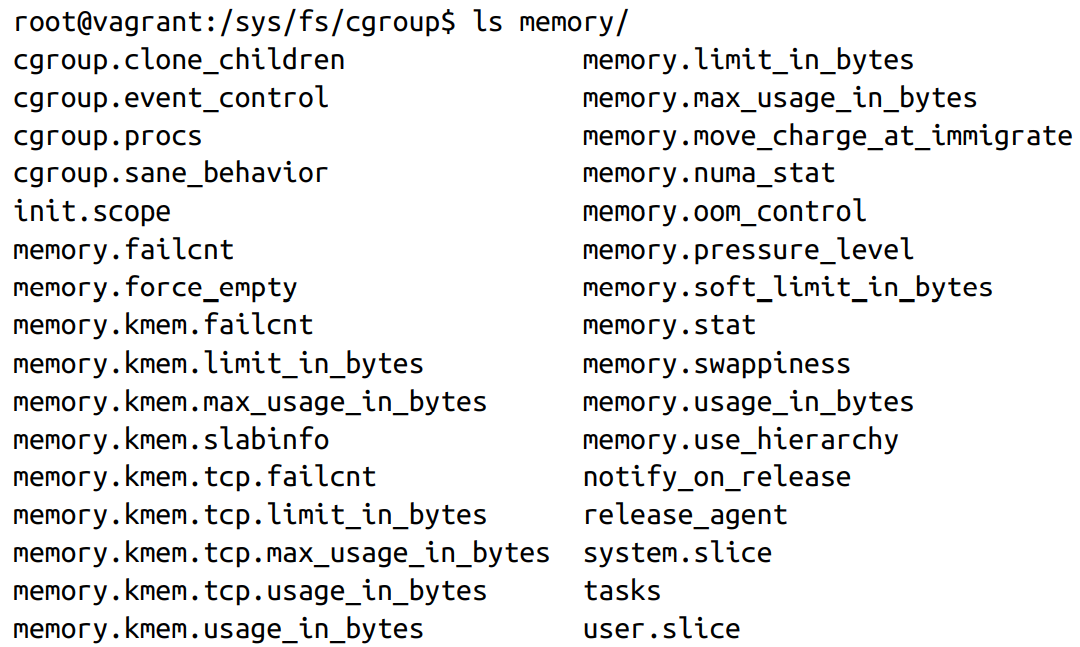
\includegraphics[width=\textwidth, keepaspectratio]{capitoli/os_security/imgs/cgroup2.png}
\end{figure}

Alcuni di questi file sono modificabili dall'utente mentre altri contengono
informazioni, scritte dal kernel, che sono di sola lettura. Per esempio,
il file \verb|memory.limit_in_bytes| contiene un valore modificabile che serve
per impostare un limite di utilizzo della memoria disponibile ai processi del gruppo.
Invece \verb|memory.max_usage_in_bytes| contiene solo l'informazione della memoria
massima utilizzata dai processi del gruppo.
Il cgroup \verb|memory| è il più alto nella gerarchia.

\section{Creazione di un Cgroup}

Creare una sottodirectory all'interno di uno dei cgroup crea un nuovo cgroup e
verrà popolato automaticamente dal kernel con i file di configurazione che rispettano
i parametri di quel cgroup.\\
La seguente immagine mostra la creazione di un nuovo cgroup chiamato \verb|liz|
all'interno del cgroup \verb|memory|.

\begin{figure}[H]
    \centering
    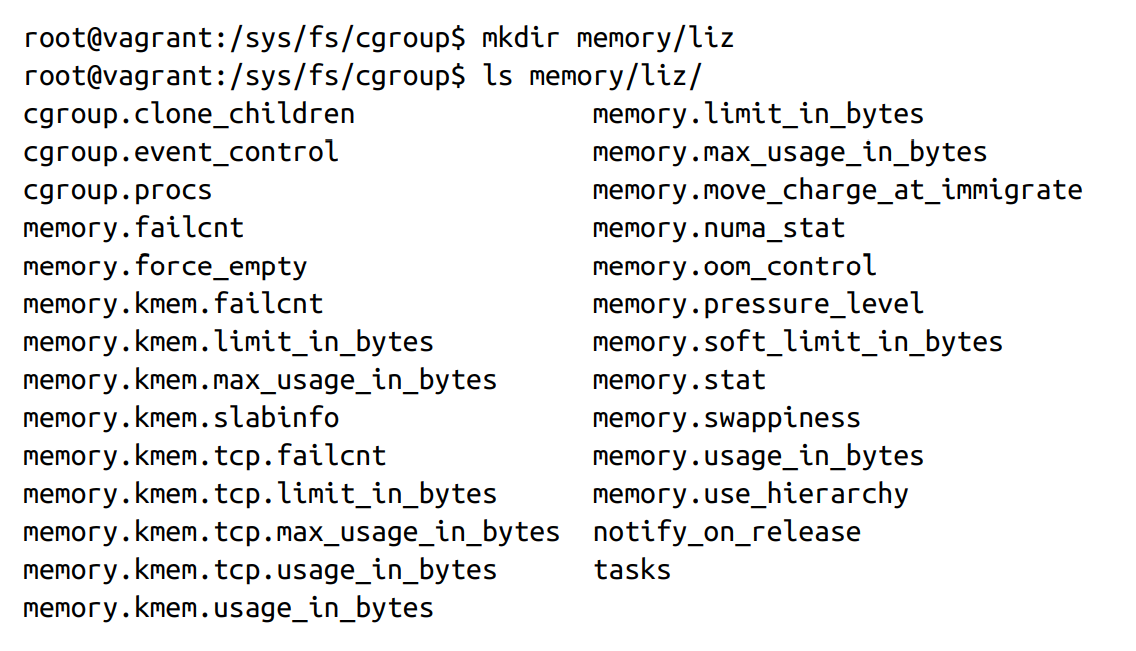
\includegraphics[width=\textwidth, keepaspectratio]{capitoli/os_security/imgs/cgroup3.png}
\end{figure}

Quando viene avviato un container, il runtime crea un nuovo cgroup appositamente
per i suoi processi. Dalla prospettiva dell'host, per vedere tutti i cgroup presenti
all'interno di un cgroup si può utilizzare il comando \verb|lscgroup|.

\begin{figure}[H]
    \centering
    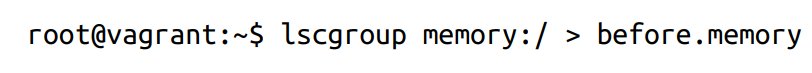
\includegraphics[width=\textwidth, keepaspectratio]{capitoli/os_security/imgs/cgroup4.png}
\end{figure}

\section{Assegnare un Processo ad un Cgroup}

Assegnare un processo ad un cgroup consiste semplicemente nello scrivere il suo
process ID nel file \verb|cgroup.procs| relativo al cgroup.

\begin{figure}[H]
    \centering
    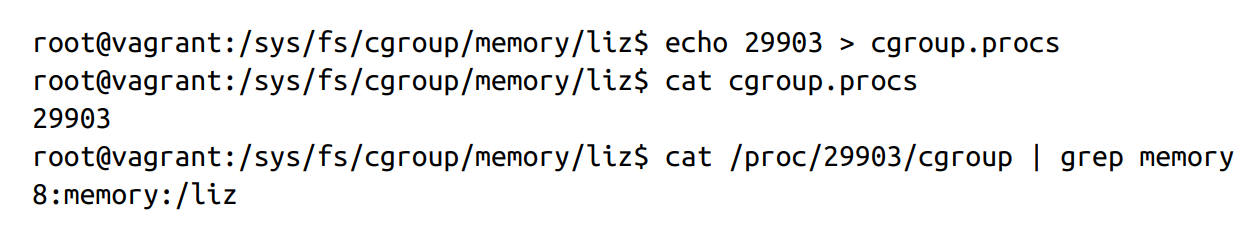
\includegraphics[width=\textwidth, keepaspectratio]{capitoli/os_security/imgs/limit4.png}
\end{figure}

\section{Limiting Resources}

Come gìa detto, per vedere quanta memoria ha a disposizione il gruppo, si può
esaminare il contenuto del file \verb|memory.limit_in_bytes|.

\begin{figure}[H]
    \centering
    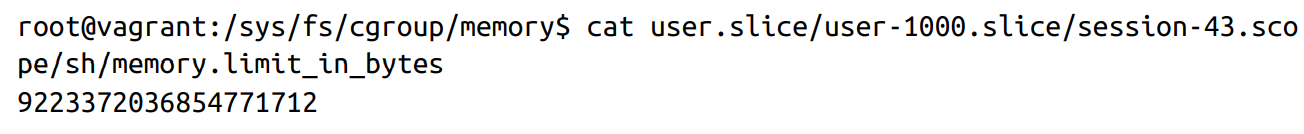
\includegraphics[width=\textwidth, keepaspectratio]{capitoli/os_security/imgs/limit1.png}
\end{figure}

Di default non è limitata come si vede dal numero enorme dell'immagine precedente.
Questa cosa non va bene dato che un processo potrebbe consumare tutta la memoria
dell'host e mandare in \textit{starving} altri processi. Ciò potrebbe essere
anche non intenzionale a causa di un \textit{memory leak} o come risultato di
un attacco di tipo \textit{resources exhaustion}. Dunque è importante impostare
dei limiti alla memoria e alle altre risorse a cui il processo può accedere.\\

Vediamo ora come impostare questi limiti in diversi casi d'uso.

\paragraph{runc.}
Modificando il file \verb|config.json| nel bundle di runtime di \verb|runc|, si può
limitare la memoria che esso assegnerà ai cgroup quando crea un container.
I limiti dei cgroup si possono configurare come segue:

\begin{figure}[H]
    \centering
    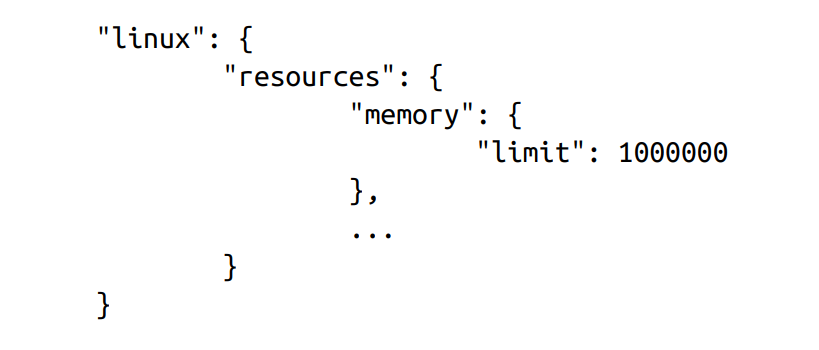
\includegraphics[width=10cm, keepaspectratio]{capitoli/os_security/imgs/limit2.png}
\end{figure}


\paragraph{docker container.} In docker può essere specificato come parametro quando
si crea un container utilizzando come parametro il flag \verb|--memory <mem limit>|.

\begin{figure}[H]
    \centering
    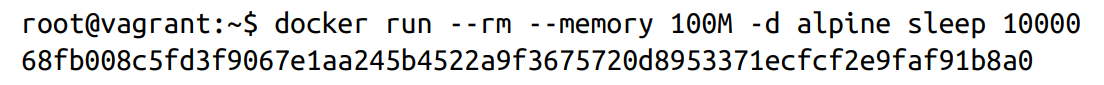
\includegraphics[width=\textwidth, keepaspectratio]{capitoli/os_security/imgs/limit3.png}
\end{figure}


\paragraph{manual.} È possibile modificare manualmente il parametro
\verb|memory.limit_in_bytes| come nel seguente esempio:

\begin{figure}[H]
    \centering
    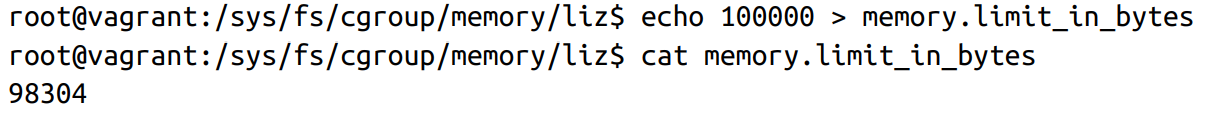
\includegraphics[width=\textwidth, keepaspectratio]{capitoli/os_security/imgs/limit5.png}
\end{figure}

\section{Docker e Cgroup}

Docker crea automaticamente i suoi cgroup di ogni tipo che possono essere osservati
cercando la directory chiamata \verb|docker| all'interno dei cgroup.

\begin{figure}[H]
    \centering
    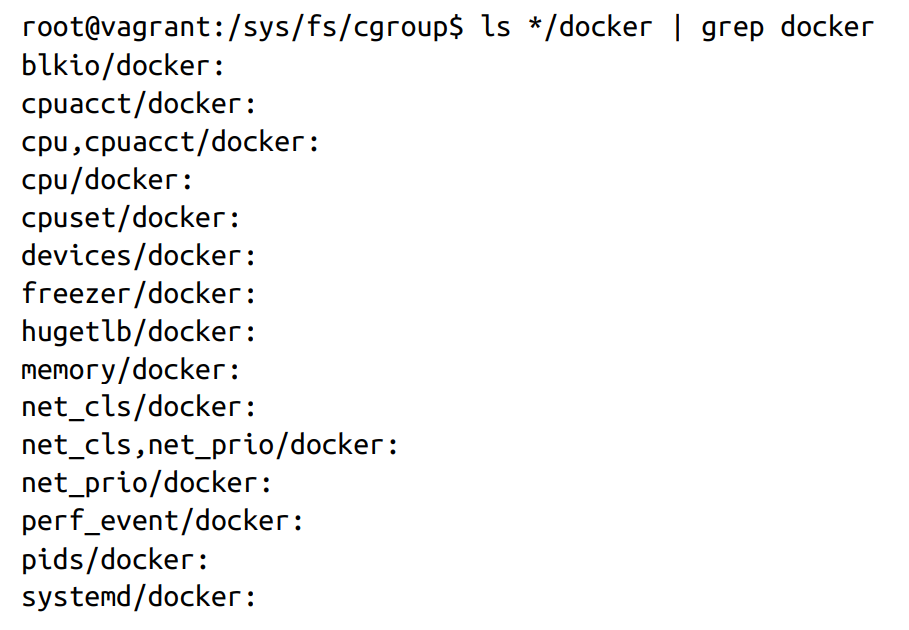
\includegraphics[width=\textwidth, keepaspectratio]{capitoli/os_security/imgs/docker1.png}
\end{figure}

Quando viene avviato un container, docker crea in automatico un altro set di cgroup
all'interno dei cgroup docker.

\section{Cgroup v2}

Cgroup v2 è la versione di cgroup introdotta dal kernel linux rilasciato nel 2016.
Tuttavia non è ancora oggi la versione più popolare. La differenza principale
è che in cgroup v2 il processo non può joinare gruppi differenti con controllori
differenti. Cgroup v2 risulta avere un supporto migliore per i container rootless
affinché possano essere applicate le limitazioni delle risorse.